\section{Einleitung}
In diesem Versuch wird ein LC-Modulator auf verschiedene Eigenschaften untersucht. LC-Modulatoren bieten die Möglichkeit schaltbar diffraktive optische Elemente zu realisieren. Durch Anlegen einer Spannung an den Flüssigkristallen im LC-Modulator können verschiedene optische Phänomene hervorgerufen werden. So ist es möglich optische Werkzeuge, wie zum Beispiel Gitter, Spalten oder Linsen realisieren. Außerdem wird der LC-Modulator auch auf seine Eigenschaften zur Amplitudenmodulation und computergenerierten Holografie überprüft.
\section{Amplitudenmodulation und Projektion}
\subsection{Winkelverteilung von linear polarisiertem Licht}
Zuerst wird der Versuch nach \cref{411} aufgebaut. Der Laser zeigt dabei entlang des Strahlengangs, auf dem auch die anderen Objekte angebracht sind. Die Linse fokussiert dabei den Laserstrahl auf das Intensitätsmessgerät.
Die Brennweite beträgt 160mm. 

\begin{figure}[h!]
	\centering
	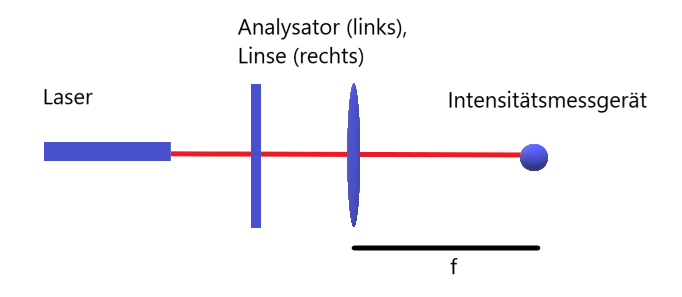
\includegraphics[scale=1]{4.1.1-Aufbau.png}
	\caption{Aufbau zur Untersuchung von Amplitudenmodulation und Projektion}
	\label{411}
\end{figure}

Zunächst wird die Polarisationsrichtung des Lasers bestimmt, indem der Analysator so eingestellt wird, dass die größte Intensität gemessen werden kann. Von diesem Punkt aus wird in 10° Schritten der Analysator gedreht und jeweils die Intensität gemessen. Dabei ergibt sich \cref{Malus}, wobei erkennbar ist, dass  sich die Intensität wie zu erwarten nach dem Gesetz von Malus verhält, welches besagt, dass 
\begin{equation}
	I = I_{0}*cos(\alpha)^{2}
\end{equation}
ist.$\alpha$ ist dabei der Winkel zwischen Polarisator und Polarisation des Lasers. In diesem Fall ist die Funktion allerdings um den Startwinkel, die der Laser zum Analysator hat, verschoben.
Nach unserer Messung lag dieser bei $\beta = \SI{45 \pm 1}{^\circ}$ im Vergleich dazu liegt der Fit bei $\beta = \SI{43,5 \pm 0,3}{^\circ}$. Das bedeutet, dass das Maximum und Minimum wahrscheinlich nicht perfekt getroffen wurde.

\begin{figure}[h!]
	\centering
	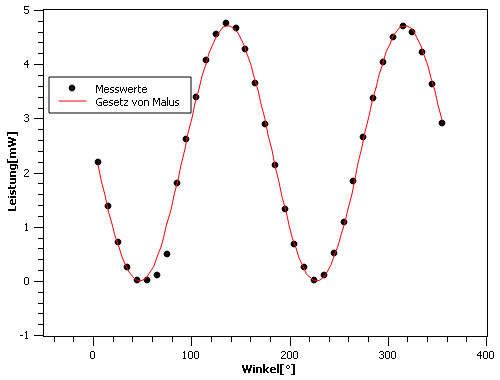
\includegraphics[scale=0.8]{GesetzvonMalus.png}
	\caption{Intensität unter verschiedenen Winkeln des Analysators}
	\label{Malus}
\end{figure}

Daraufhin können die maximal und minimale gemessene Intensität verglichen werden, um den Kontrast zu bestimmen:
\begin{equation}
	C = \frac{I_{max} - I_{min}}{I_{max} + I_{min}} = \SI{0,9943 \pm 0,0004}{}
	\label{eq:Kontrast}
\end{equation}


\subsection{Vorbereitungen zur optimierten Funktion des LC-Modulators}
Der nächste Versuch wird nach \cref{412} aufgebaut. Da die Polarisation des Lasers jetzt bekannt ist, kann er so gedreht werden, dass sie im -45° Winkel zum LC-Modulator liegt, da er dort den maximalen Kontrast hat. Hinter dem LC-Modulator folgt ein Analysator, der auf einen Polarisationswinkel von -135° eingestellt werden soll. Mit der Kamera kann das Bild beobachten werden.

\begin{figure}[h!]
	\centering
	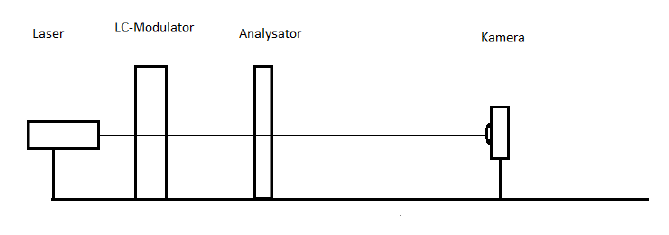
\includegraphics[scale=1]{4.1.2-Aufbau.png}
	\caption{Aufbau zur Variation des Kontrasts}
	\label{412}
\end{figure}

Als nächstes wird der LC-Modulator angesteuert, sodass die eine Seite des Bildschirms schwarz ist und die andere weiß. Dabei werden vier Bilder gemacht, wobei der Analysator jeweils um 45° weiter gedreht wird, wie sie auch in \cref{Kontrast} zu sehen sind. 

\begin{figure}
	\begin{subfigure}[]{0.5\textwidth}
		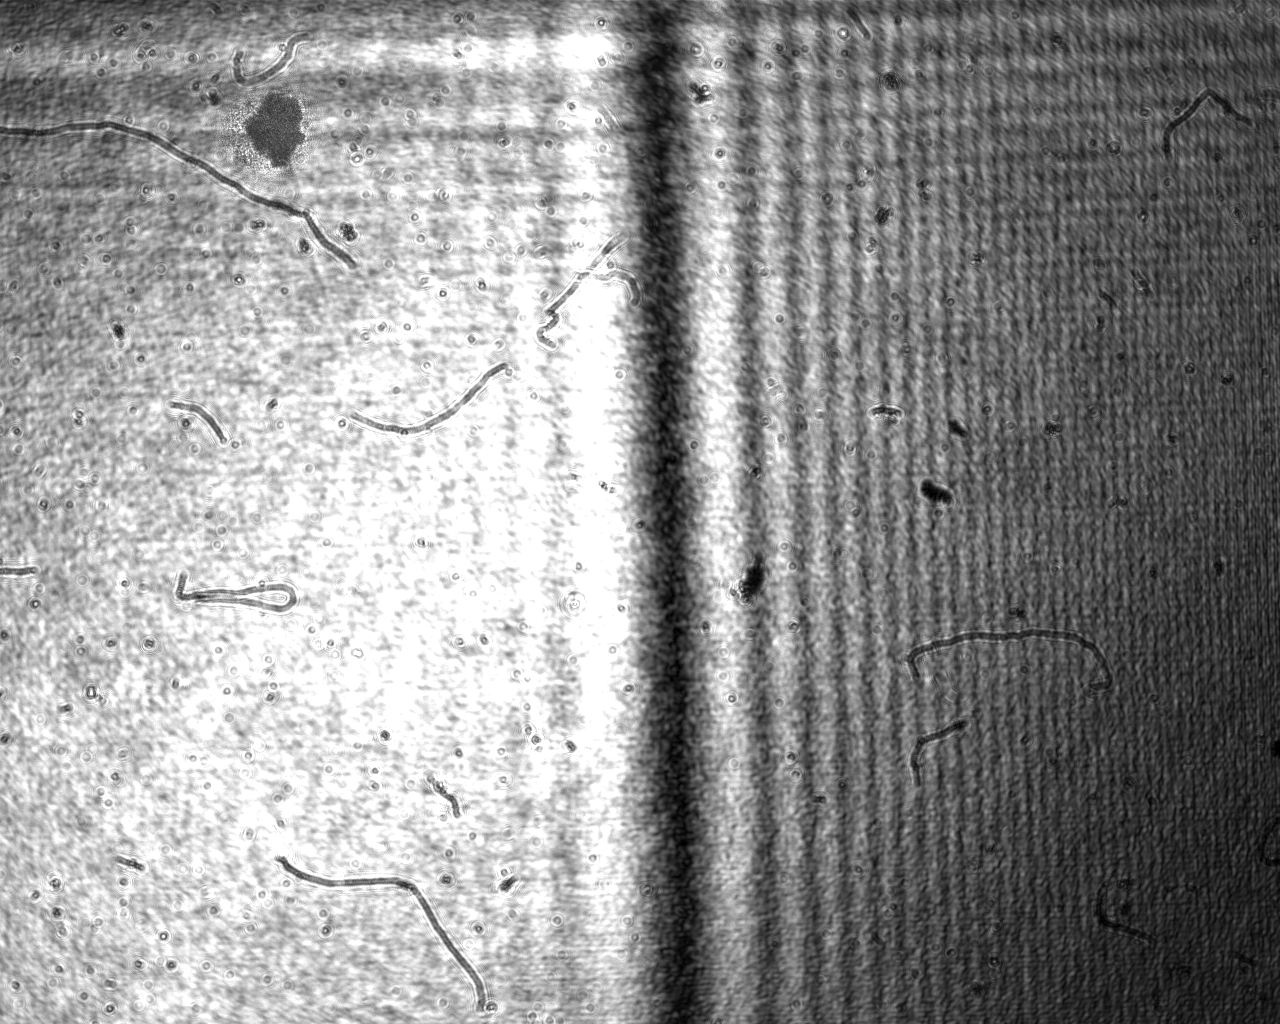
\includegraphics[width=0.6\textwidth]{4.1.2_0Grad.png}
		\caption{0° gedreht}
	\end{subfigure}
	\begin{subfigure}[]{0.5\textwidth}
		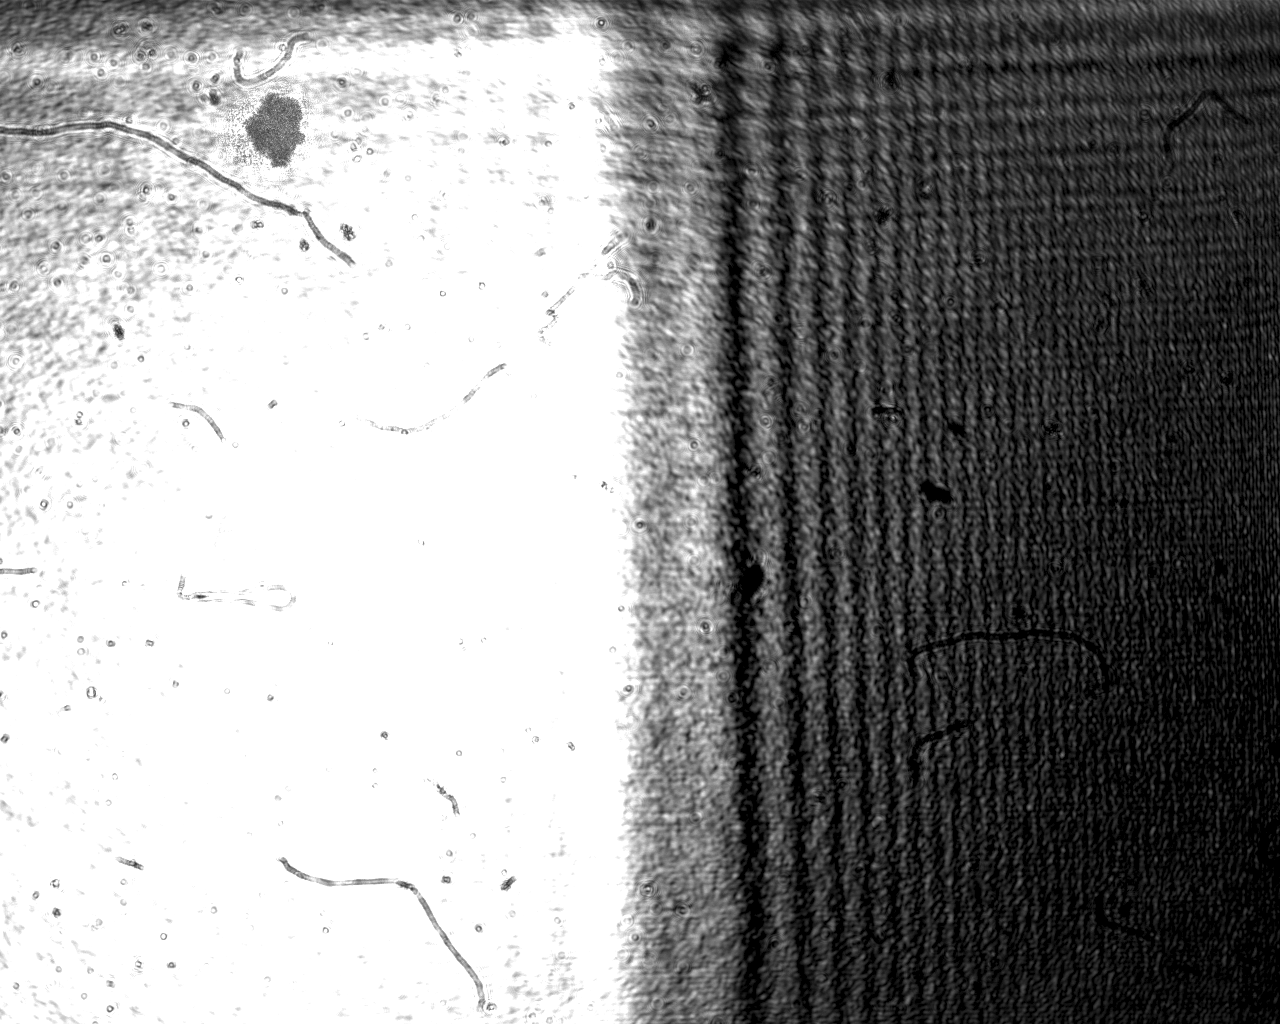
\includegraphics[width=0.6\textwidth]{4.1.2_45Grad.png}
		\caption{45° gedreht}
		\label{45}
	\end{subfigure}


	\begin{subfigure}[]{0.5\textwidth}
		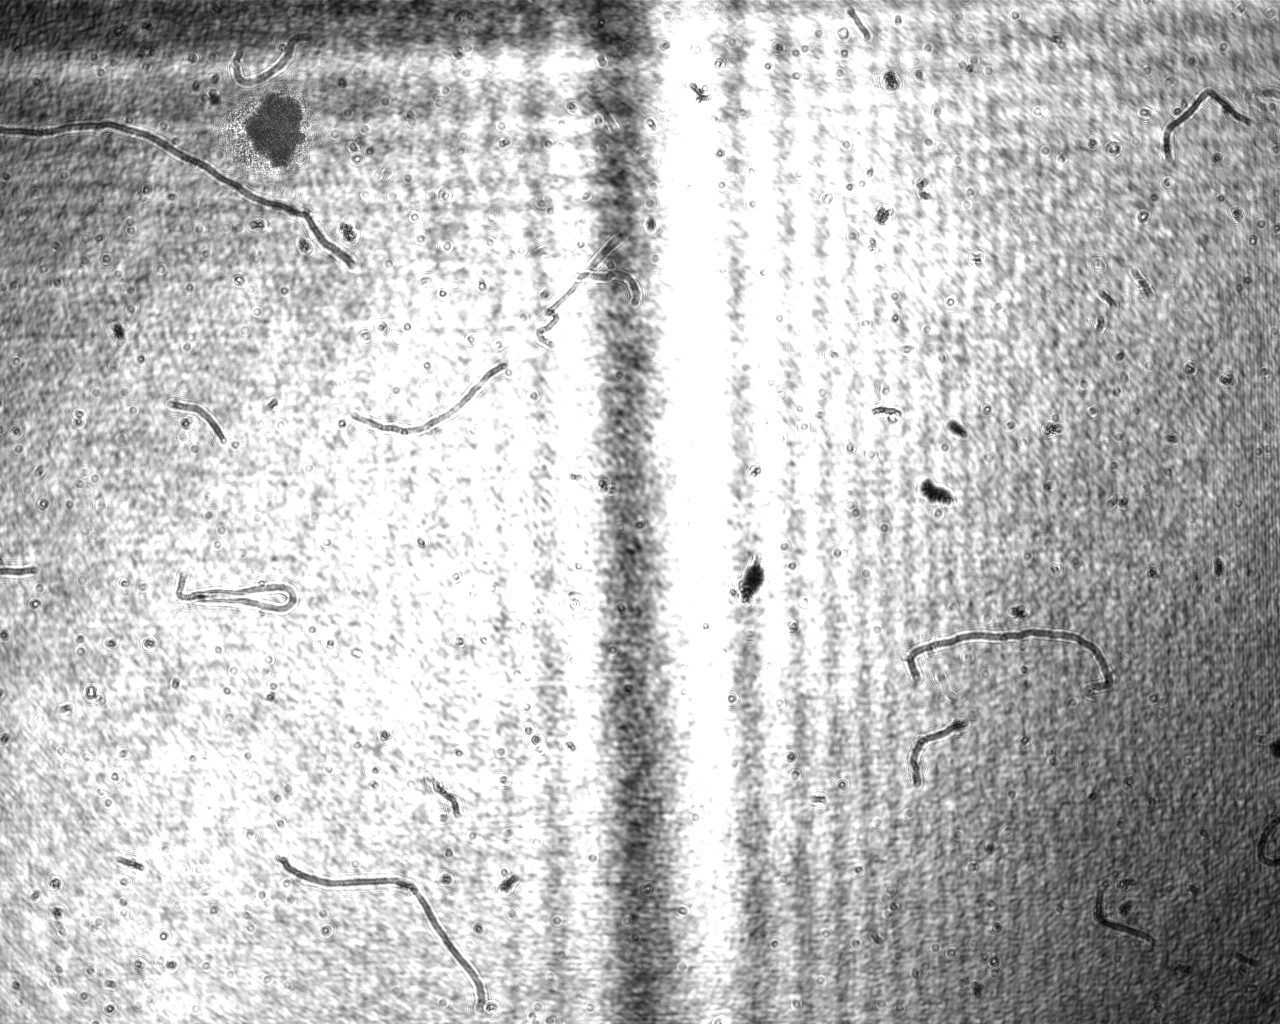
\includegraphics[width=0.6\textwidth]{4.1.2_90Grad.png}
		\caption{90° gedreht}
	\end{subfigure}
	\begin{subfigure}[]{0.5\textwidth}
		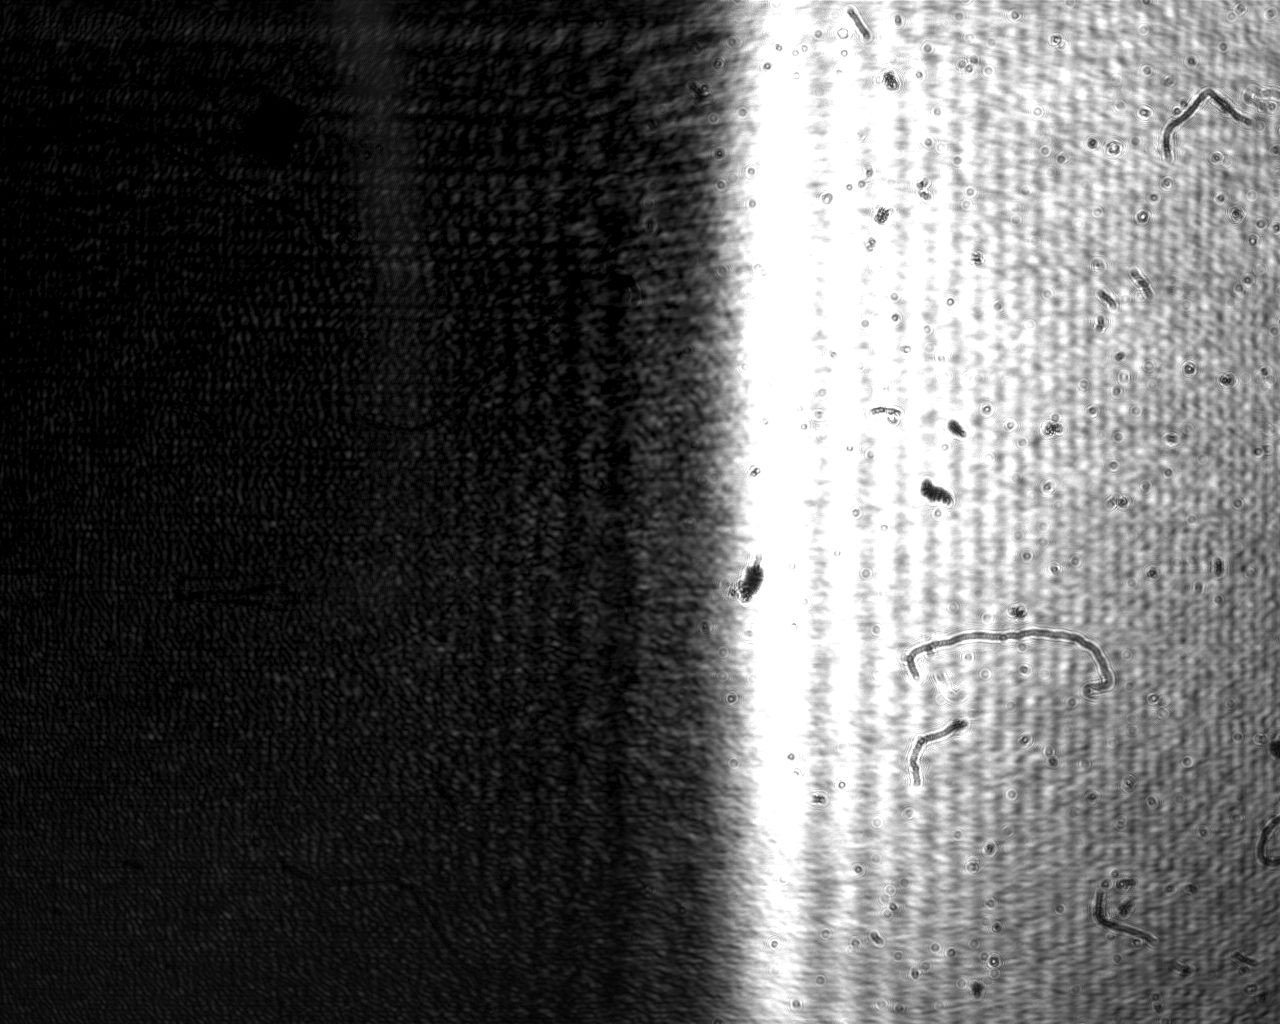
\includegraphics[width=0.6\textwidth]{4.1.2_135Grad.png}
		\caption{135° gedreht}
		\label{135}
	\end{subfigure}
	\caption{Bilder unter verschiedenen Einstellung des Analysators}
	\label{Kontrast}
\end{figure}

Dabei wird deutlich, dass die Bilder \cref{45} und \cref{135} genau die invertierten voneinander sind. Die beiden anderen Bilder ähneln sich sehr stark. Somit wird klar, dass sich der Kontrast mit der Stellung des Analysators ändert, wobei 45° die optimale Einstellung ist und für den Rest des Versuches beibehalten wird. 

Daraufhin wird die Kamera mit einer Linse und dem Intensitätsmessgerät ersetzt. Bei dem LC-Modul, wird ein rein weißer bzw. schwarzer Bildschirm statt des geteilten benutzt. Für diese beiden Konfigurationen wird jeweils eine Intensitätsmessung durchgeführt, welche ergeben haben: $I_{max} = \SI{1,336}{mW}$ und $I_{min} = \SI{0,106}{mW}$. Daraus folgt mit \cref{eq:Kontrast} ein Kontrast von C = 0,853, was deutlich niedriger als der vorherige Kontrast ist. 
Das lässt sich damit erklären, dass der LC-Modulator auch als Phasenmodulator fungiert, was den Kontrast verschlechtert.

Die Änderung der Polarisation liegt am Aufbau des LC-Modulators bzw. der einzelnen Zellen. Eine schematische Aufzeichnung davon ist in \cref{LC-Modul} zu sehen. Bei keiner angelegten Spannung sind die einzelnen Moleküle in einer Raumrichtung leicht zueinander verschoben, wodurch sich langsam  bei jedem Schritt die Polarisation ändert, 
bis sie 90° erreicht hat. Bei einem schwachem angelegten Feld sind die Moleküle zudem noch in eine Zweite Raumrichtung ineinander verdreht. Erst sobald ein gewisser Grenzwert erreicht wird, richten sich die Moleküle vollkommen parallel zueinander aus, bis auf die Moleküle an der Endfläche, und ändern die Polarisation gar nicht mehr. 


\begin{figure}[h!]
	\centering
	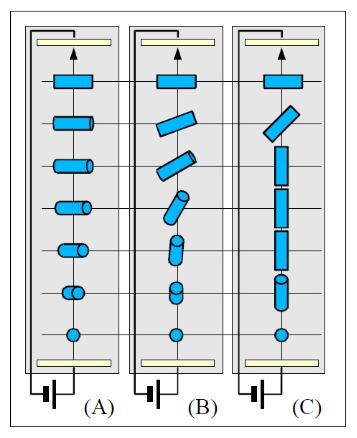
\includegraphics[scale=0.6]{LC-Zelle.png}
	\caption{Verhaltensweise einer Flüssigkristallzelle bei verschiedenen Spannung. a) Keine Spannung b) Spannung unter Grenzwert c) Spannung über Grenzwert}
	\label{LC-Modul}
\end{figure}

\subsection{Pixelgröße des LC-Displays}
Als nächstes soll die Pixelgröße des Displays bestimmt werden. Dafür wird der Versuch nach \cref{413} aufgebaut. Dabei hat die Linse eine Brennweite von $f = \SI{16}{cm}$ und der Schirm ist b = $\SI{78,5 \pm 0,2}{cm}$ von der Linse entfernt. Daraufhin wird ein weißes Bild mit einem 200 x 200 großen schwarzen Quadrat an den LC-Modulator adressiert und die Bildgröße mit einem Lineal auf dem Schirm gemessen. Diese ist auf $B = \SI{2,6 \pm 0,3}{cm}$
bestimmt worden.
\begin{figure}[h!]
	\centering
	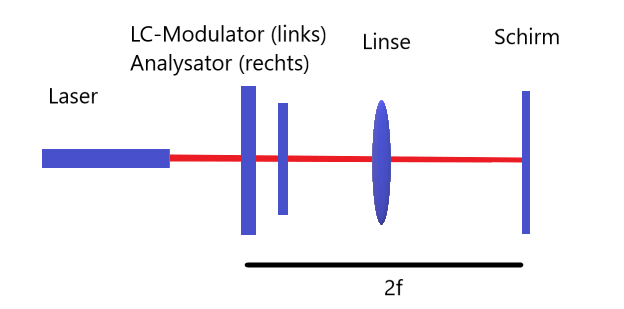
\includegraphics[scale=1]{4.1.3-Aufbau.png}
	\caption{Aufbau zur Bestimmung der Pixelgröße}
	\label{413}
\end{figure}

Die Pixelgröße kann dann über die Formel
\begin{equation}
	G = \frac{B}{\frac{b}{f} - 1} 
\end{equation}
berechnet werden. Da das benutzte Quadrat eine Pixelgröße von 200 Pixeln hat , muss die Formel noch durch 200 geteilt werden um  auf das Endergebnis mit $G = \SI{33 \pm 1}{\mu m}$ zu kommen. 

\subsection{Zusammenhang zwischen Grauwert und Polarisationszustand}
Im nächsten Versuchsteil soll der Zusammenhang zwischen Grauwert und Polarisationszustand behandelt werden. Dazu wird der Versuch, wie in \cref{414} gezeigt, aufgebaut. Dabei werden verschiedene Grauwerte eingestellt und die maximale und minimale Intensität, bei verschiedenen Einstellungen des Analysators, sowie der dazugehörige Winkel aufgeschrieben. Diese Messungen sind in \cref{tab:grauwert} zu sehen.


\begin{figure}[h!]
	\centering
	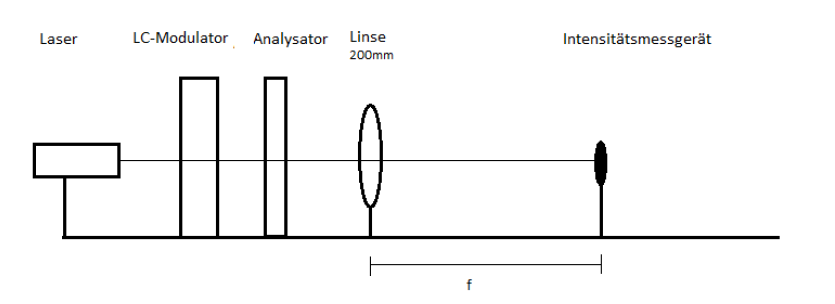
\includegraphics[scale=1]{4.1.4-Aufbau.png}
	\caption{Aufbau zur Erforschung zum Zusammenhang zwischen Grauwert und Polarisationszustand}
	\label{414}
\end{figure}

\begin{table}[]
	\caption{Messung der intensität für verschiedene Grauwerte }
	\label{tab:grauwert}
	\begin{tabular}{l|llll}
		Graustufen & max Winkel & max Intensität & min Winkel & min Intensität \\ \hline
		0          & 50         & 1              & 140        & 0,014          \\
		50         & 50         & 0,985          & 145        & 0,036          \\
		100        & 59         & 0,923          & 148        & 0,075          \\
		150        & 103        & 0,869          & 195        & 0,186          \\
		200        & 123        & 0,968          & 211        & 0,03           \\
		250        & 123        & 0,98           & 212        & 0,028         
	\end{tabular}
\end{table}



Die Grauwerte entsprechen dabei einer angelegten Spannung am LC-Modulator. Da dieser aus Twisted nematic Flüssigkristallzellen besteht, die bei nicht angelegter Spannung die Polarisation des Lasers um 90° drehen und der Laser immer noch in die -45° Richtung polarisiert ist, scheint es klar zu sein, dass bei einer Graustufe von 0 auch keine Spannung angelegt wird. Sobald eine bestimmte Spannung am LC-Modulator überschritten ist, ändert dieser auch die Polarisation des Lichts nicht mehr. Auch das stimmt näherungsweise mit den Messwerten überein. Wie in \cref{tab:grauwert} zu sehen ist, wird bei einem fast maximalem Grauwert von 250(Maximum ist bei 255), auch wieder eine ähnliche Polarisation, wie sie der Laser am Anfang hat, vorgefunden. 

Es ist möglich die Exzentrizität des Lichts bildlich zu bestimmen, indem die maximale Intensität als die große Halbachse und die minimale Intensität, als die kleine Halbachse einer Ellipse angesehen werden. Der Winkel der maximalen Intensität entspricht dabei der Drehung der Ellipse. Beispielhaft ist das für einige ausgewählte Grauwerte in \cref{Ellipse} zu sehen. Dabei wird besonders deutlich, dass der maximale und minimale Grauwert um annähernd 90° zueinander gedreht sind, wie es auch erwartet wurde.

\begin{figure}[h!]
	\centering
	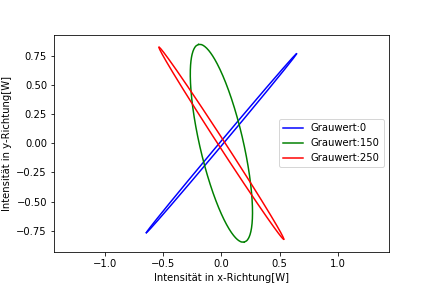
\includegraphics[scale=0.6]{Ellipse.png}
	\caption{Exzentrizität des Lichts für ausgewählte Grauwerte}
	\label{Ellipse}
\end{figure}





\section{LC-Modulator als DOE}
\subsection{Berechnung der Pixelgröße}
\subsubsection{Theorie}
Zur Bestimmung der Breite eines Pixels innerhalb des LC-Modulators wird mit der Formel eines Gitters gerechnet, da ein LC-Modulator dasselbe Beugungsbild aufweißt.
\begin{align}
	g\sin{\alpha} = m\lambda
	\label{gbestimm}
\end{align}
Dabei stellt g die Gitterkonstante, $\alpha$ den Winkel zwischen der nullten und m-ten Beugungsordnung, m die entsprechende Beugungsordnung und $\lambda$ die Wellenlänge des Lasers ($\lambda = 650nm$) dar.
Die Bestimmung von $\alpha$ kann aus der Optik durch
\begin{align}
	\alpha \approx \frac{d}{2f}
	\label{abestimm}
\end{align}
berechnet werden. Dabei ist d der Abstand zweier gleicher höherer Ordnungen. 
\subsubsection{Aufbau}
Der Aufbau zur Berechnung der Pixelgröße ist in \cref{421} dargestellt.
Zuerst wird der Laser auf einen LC-Modulator gerichtet, welcher in dem Abstand der Brennweite der Linse ($f = 16cm$) von der Linse entfernt steht. Zwischen der Linse und dem LC-Modulator ist ein Analysator. Hinter der Linse ist im Abstand ihrer Brennweite ein Schirm aufgestellt, um die Beugungsordnungen messen zu können. 
\begin{figure}[h!]
	\centering
	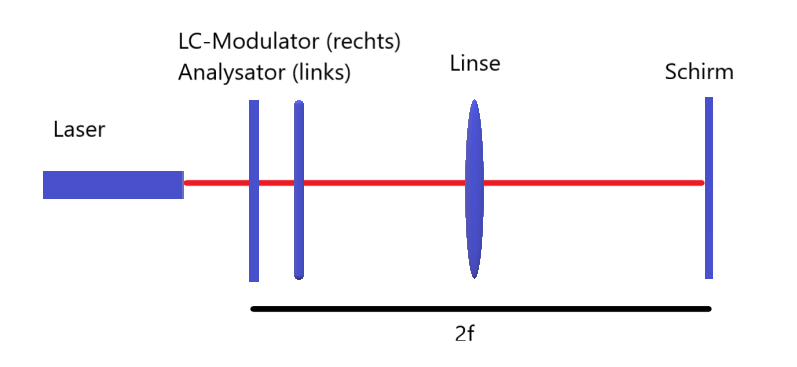
\includegraphics[scale = 1]{4.2.1-Aufbau.png}
	\caption{Aufbau zur Bestimmung der Pixelgröße}
	\label{421}
\end{figure}
\subsubsection{Auswertung}
Um \cref{gbestimm} möglichst genau zu berechnen, wurde bei der Berechnung von \cref{abestimm} der Abstand der siebten Ordnungen benutzt, um d zu messen. Dieser Abstand wurde mittels eines Lineals gemessen. Aus diesen Berechnungen kann die Gitterkonstante bestimmt werden $g = (29 \pm 3) \mu m$.
\subsubsection{Unsicherheiten}
Die Unsicherheit von d wurde mit einer Genauigkeit von $\pm 0,2cm$ angenommen. Daraus resultiert für die Unsicherheit der Gitterkonstanten mittels Fehlerfortpflanzung ein Wert von $g = (29 \pm 3) \mu m$.
\subsubsection{Diskussion}
Somit liegt das Ergebnis der Pixelgröße von $g = (29 \pm 3) \mu m$ innerhalb der angegebenen Pixelgröße von $g = 32 \mu m$. In Aufgabenteil 1.3 Pixelgröße eines LC-Displays wurde die Größe eines Pixels auf $g = (33 \pm 1) \mu m$ gemessen. Ebenfalls diese beiden Ergebnisse stimmen in Abhängigkeit der Unsicherheiten miteinander überein.

\subsection{Intensitätsverteilung in den Beugungsordnungen des unadressierten Displays}
\subsubsection{Theorie}
Eine LCD-Zelle besitzt eine Untermodulation. Dies ist deshalb der Fall, da in einem einfachen Pixel es einen transparenten Anteil gibt, sowie einen lichtundurchlässigen Anteil. Die Modulation wird durch das Gitter beschrieben, welches im vorherigen Aufgabenteil behandelt wurde. Die Untermodulation wird durch die Substruktur im Pixel erzeugt. An dieser Stelle wird der duty cycle definiert. Dieser beschreibt das Verhältnis zwischen transparentem und lichtundurchlässigem Teil. Der Füllfaktor kann ebenfalls an dieser Stelle definiert werden. Dieser entspricht gerade dem Anteil des durchlässigen Pixels zur Gesamtpixelgröße.
Anhand von \cref{gesh} können die Formeln für den duty cycle und den Füllfaktor veranschaulicht werden. abei stellt das Quadrat ein Pixel dar. Das schwarze Rechteck ist dabei der lichtunduchlässige Teil, wohingegen der noch vorhandene Teil den lichtdurchlässigen Anteil darstellt
Dabei steht x für die Breite des Undurchlässigen Anteils des LC-Modulators und y steht für die Höhe des undurchlässigen Anteils des LC-Modulators.
Die Breite des Pixels ist g.
\begin{figure}[h!]
	\centering
	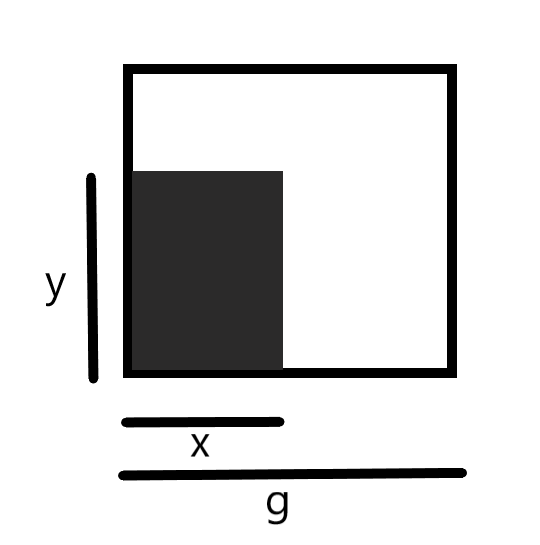
\includegraphics[scale = 1]{dutyyy.png}
	\caption{Schematische Darstellung zur Berechnung des duty cycle und des Füllfaktors.}
	\label{gesh}
\end{figure}
Der duty cycle wird berechnet, indem sinc-Funktionen an die Untermodulation angepasst werden. Die Breiten der sinc-Funktionen entsprechen dann dem durchlässigen Anteil in der jeweiligen Richtung. 
Der duty cycle ergibt sich dann durch
\begin{align}
	\text{duty cycle} = \frac{xy}{g^{2}-xy}
	\label{dutycyc}
\end{align}
Ebenfalls kann auf den Füllfaktor geschlossen werden für den transparenten Teil des Pixels. 
\begin{align}
	\text{Füllfaktor} = \frac{xy}{g^{2}}
	\label{ff}
\end{align}

\subsubsection{Aufbau}
Der Aufbau zur Berechnung des Füllfaktors der LCD-Zelle ist in \cref{422} dargestellt. Zuerst wird der Laser, welcher eine zusätzlich integrierte Aufweitungsoptik besitzt auf das LCD-Display gerichtet. Danach wird ein Analysator in den Strahlengang geführt. Statt einem Schirm wird die Auswertung mit einem Intensitätsmessgerät durchgeführt.
\begin{figure}[h!]
	\centering
	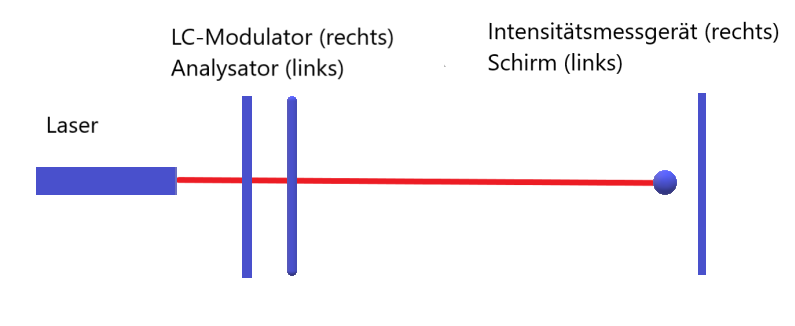
\includegraphics[scale = 1]{4.2.2-Aufbau.png}
	\caption{Aufbau zur Bestimmung des Füllfaktors der LCD-Zellen}
	\label{422}
\end{figure}
\subsubsection{Auswertung}
Im weiteren wurden die ersten zehn Beugungsordnungen in horizontaler und vertikaler Ebene gemessen. Die Messwerte sind in \cref{horiz} zu sehen.
\begin{figure}[h!]
	\centering
	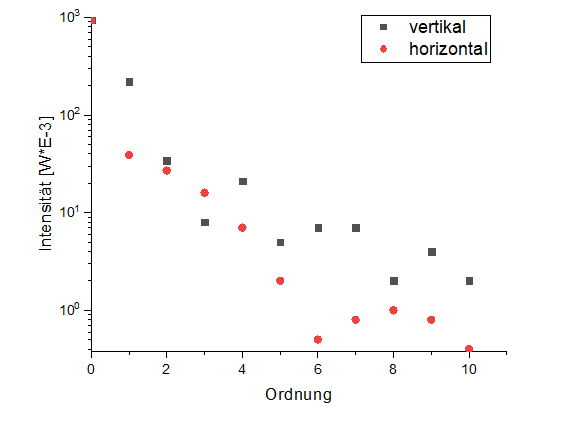
\includegraphics[scale = 1]{horizundvertik.png}
	\caption{Intensitätsverteilung der horizonatlen und vertikalen Beugungsordnungen}
	\label{horiz}
\end{figure}
Aus den Messwerten kann auf den duty cycle geschlossen werden, sowie auf den Füllfaktor des transparaneten Teils der LCD-Zelle in Bezug auf das Gesamte Pixel. Um den duty cycle zu berechnen wird \cref{dutycyc} benutzt. Hierfür werden die Breiten der sinc-Funktionen nicht durch den Fit bestimmt, welcher aufgrund der wenigen Messdaten nicht funktioniert hat, sondern es wird visuell das Minimum der sinc-Funktionen gesucht und damit den Stauch- bzw. Streckfaktor innerhalb der sinc-Funktion berechnet. Über einen Vergleich des Stauchfaktors kann die Breite des Peaks entnommen werden.
Daraus ergibt sich ein duty cycle und ein Füllfaktor von 
\begin{align}
	\text{duty cycle} = (0,59 \pm 0,11)\% \\
	\text{Füllfaktor} = (1,47 \pm 0,8)\%
\end{align}
\subsubsection{Unsicherheiten}
Die Unsicherheiten wurden mittels Fehlerfortpflanzung berechnet. Es wurden dieselben Unsicherheiten benutzt, die in 2.1 Berechnung der Pixelgröße verwendet wurden.
\subsubsection{Diskussion}
Der Füllfaktor, welcher durch die obige Auswertung berechnet wurde, ist gleich mit der Angabe des Herstellers, welcher in LC 2012 Spatial Light Modulator (transmissive) aufgelistet wurde. In den Angaben des Herstellers ist der Füllfaktor bei einem Wert von $58 \%$. Der oben ausgerechnete Wert unterscheidet sich innerhalb des Fehlers nicht von der Angabe des Herstellers. Ebenfalls entspricht die Pixelbreite von $g = (29 \pm 3) \mu m$ den Angaben.

\subsection{Aufnahme von verschiedenen Beugungsbildern mittels der Kamera}
\subsubsection{Theorie}
Der Beugungswirkungsgrad $\nu$ einer DOE-Zelle bei einem vorgegebenen Grauwert ist durch folgende Formel definiert.
\begin{align}
	\nu = \frac{I_\text{1,max}}{I_\text{0,max}}
	\label{fff}
\end{align}
Der Beugungswirkungsgrad ist je nach eingestelltem Grauwert unterschiedlich. Der Grauwert wird in der DOE-Zelle eingestellt.
\subsubsection{Aufbau}
Der Aufbau in \cref{423} ist identisch mit dem Aufbau in \cref{421} mit dem Unterschied, dass statt des Schirms eine Kamera integriert wurde.
\begin{figure}[h!]
	\centering
	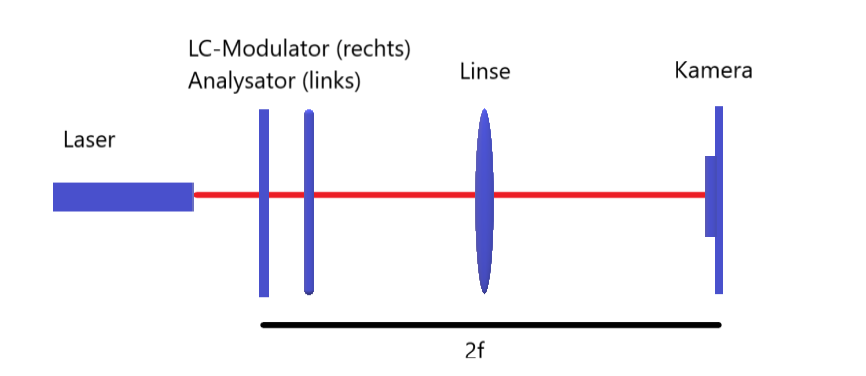
\includegraphics[scale = 1]{Kamera111.png}
	\caption{Aufbau zur Aufnahme von Beugungsbildern, die von dem LC-Modulator erzeugt werden mit Hilfe einer Kamera.}
	\label{423}
\end{figure}
\subsubsection{Auswertung}
In diesem Teil werden Beugungsbilder verschiedener DOE's aufgenommen. Darunter befinden sich der Einzelspalt, der Doppelspalt und das Gitter. Bei dem Einzelspalt werden zwei verschiedene Strukturgrößen benutzt. Aufgrund der Aufnahmen die gemacht wurden, kann man nur das Hauptmaximum beobachten, sowie die Untermodulation. Die Nebenmaxima, welche dieselbe Form haben,welche vertikal und horizonatal verschoben und dunkler sind, können nicht beobachtet werden. 
Einmal wurde eine Dicke des Spaltabstandes von 20 Pixeln und einmal von 40 Pixeln verwendet. Es ist zu beobachten, dass die Anzahl der Maxima in horizontaler Richtung, bei einem breiteren Spaltabstand, zunimmt. Somit können mehrere Nebenmaxima innerhalb der Untermodulation auf kleinerem Raum beobachtet werden.
\begin{figure}[h!]
	\centering
	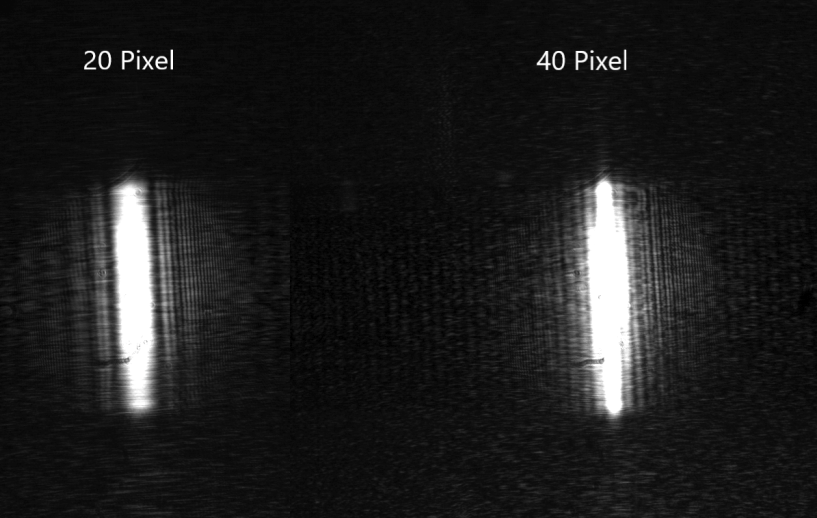
\includegraphics[scale = 1]{pixelverg.png}
	\caption{Zwei Einzelspalte. Der erste mit einer Breite von 20 Pixeln (links), der zweite mit einer Breite von 40 Pixeln (rechts)}
	\label{verg}
\end{figure}
In \cref{doppel} ist das Beugungsbild eines Doppelspaltes mit einer Breite von 30 Pixeln und einem Abstand beider Spalte von 100 Pixeln zu sehen. Es ist ein Hauptmaximum in diesem Bild zu erkennen. Innerhalb des Hauptmaximums ist ein Interferenzbild zu sehen. In der Mitte ist die Intensität (bis auf die beiden Intensitätspeaks) am stärksten und fällt zu den Seiten ab. So entspricht auch das Bild der Untermodulation dem Beugungsbild eines Doppelspaltes.
\begin{figure}[h!]
	\centering
	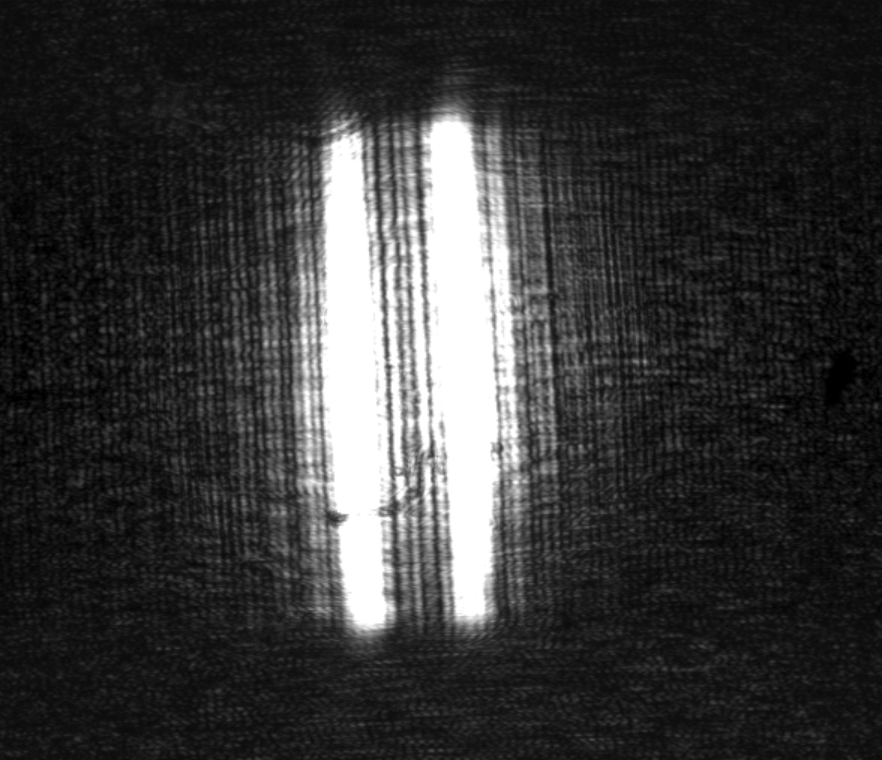
\includegraphics[scale = 0.7]{doppelspalt.png}
	\caption{Doppelspalt mit einer Breite von 30 Pixeln und einem Abstand von 100 Pixeln.}
	\label{doppel}
\end{figure}

In \cref{gitter} kann das Hauptmaxima eindeutig erkannt werden. In diesem Bild kann weiterhin statt der Untermodulation, die die ganze Zeit betrachtet wurde, das Nebenmaxima in vertikaler Richtung identifiziert werden. Beide Maxima bestehen aus Untermodulationen, was für die Nutzung einer DOE spricht.
\begin{figure}[h!]
	\centering
	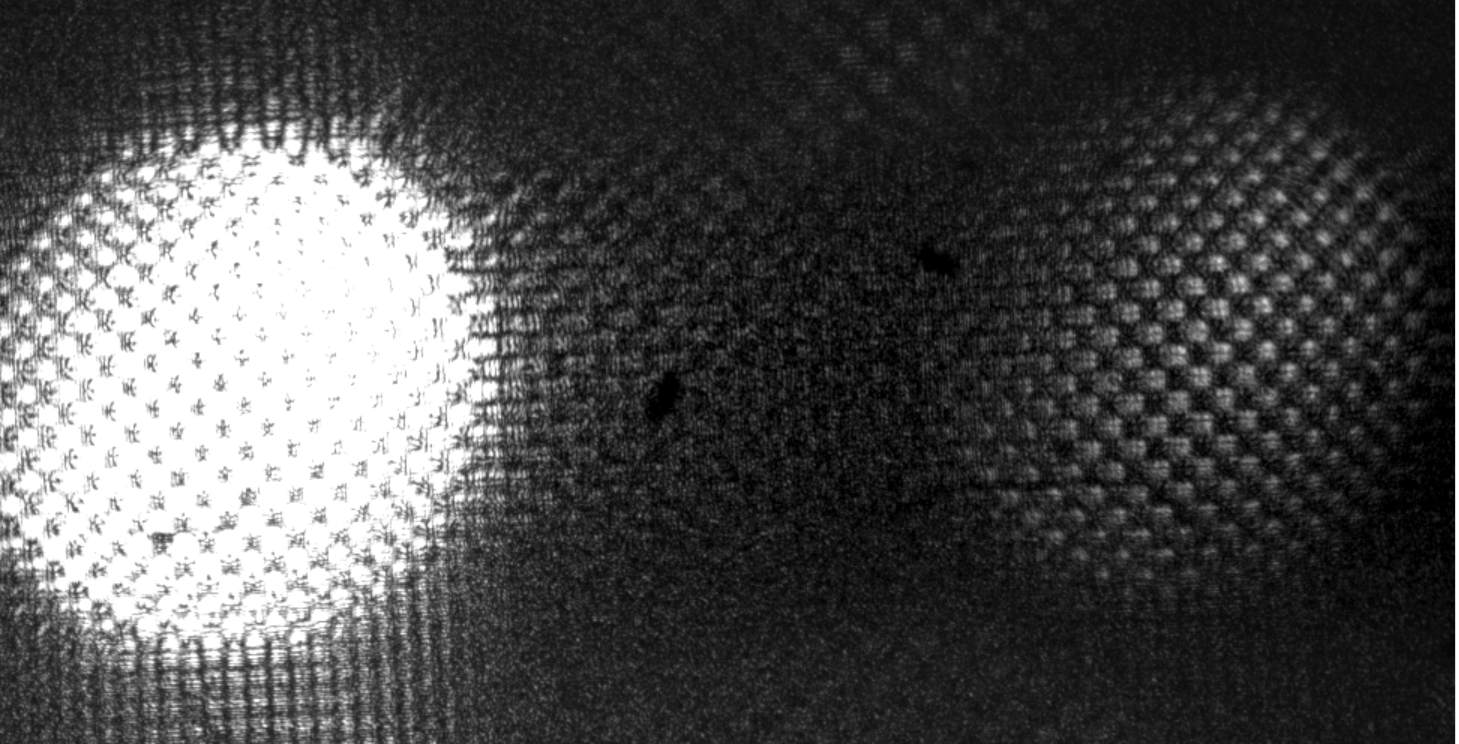
\includegraphics[scale = 0.6]{gitter.png}
	\caption{Das Beugungsbild eines Gitters in erster und zweiter Ordnung mit Beobachtbarer Untermodulation.}
	\label{gitter}
\end{figure}
Desweiteren wird für ein Grauwert die Intensitäten des 0.ten und des 1.ten Beugungsmaxima gemessen. Mittels der Intensitäten lässt sich der Beugungswirkungsgrad berechnen. Dieser wurde nur für eine Graustufe aufgenommen, sodass der Beugungswirkungsgrad bei $0,21 \pm 0,01$ bei einer Graustufe von 20 lag.

\subsubsection{Diskussion}
Das ein LC-Modulator Beugungsilder erzeugen kann leigt an der Anordnung der Flüssigkristalle. Dies ist in \cref{LC-Modul} zu sehen. Durch das Anlegen von Spannung kann eine Verkippung und eine Verdrehung erzeugt werden. Einfallendes Licht wird durch die Kristalle in ihrer Polarisation verändert. Fällt das Licht jetzt auf einen Analysator wird das Licht in abhängigkeit seiner Polarisation entweder transmittiert oder nicht transmittiert.
Der zweite wichtige Punkt ist die Größe der Pixel. Da die Größenordnung der Pixel klein genug ist, ist es möglich die Lichtwellen zur Interferenz zu bringen, falls ein Pixel mehrere Größenordnungen größer wäre, wäre es problematisch Interferenzen zu erzeugen.
Durch diese beiden Methoden ist der LC-Modulator in der Lage Beugungsbilder hervorzurufen.

\section{Computergenerierte Hologramme (CGH)}
Zuletzt wird der Aufbau, welcher in \cref{cghskizze} zu sehen ist realisiert. Das heißt LC-Modulator und Analysator in optimaler Konfiguration, eine 200mm Linse und eine Kamera zur Aufnahme der Bilder. Dieser wird für den kommenden, letzten Versuchsteil nicht mehr verändert.

\begin{figure}
	\centering
	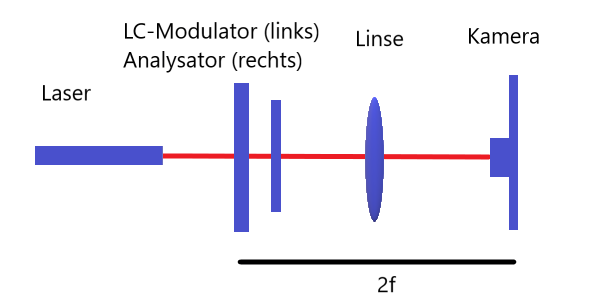
\includegraphics[scale=1]{4.1.2-Aufbau2.png}
	\caption{Aufbau des Versuchsteils zu computergenerierten Hologrammen}
	\label{cghskizze}
\end{figure}

\subsection{Brennweite der diffraktiven Linse}
Mithilfe der Software wird ein DOE in Form eines Blank Screens erzeugt. Anschließend wird eine Linsenphasenfunktion hinzuaddiert. Dies verändert den Fokus des Aufbaus, der nun neu bestimmt werden muss. Dies wird für vier verschiedene Linsenphasen (100,75,50,25) durchgeführt. Die Ergebnisse sind in \cref{tab} aufgeführt. Wie in \cref{linsenphase} erkennbar ist, verhält sich die Brennweite zur Linsenphase wie ein Wurzelfunktion.

\begin{table}[h]
	\caption{Die Brennweite für vier verschiedene Linsenphasen.}
	\begin{tabular}{ll}
		Linsenphase & Brennweite[cm]\\
		$25$ & $89\pm0,3$\\
		$50$ & $95\pm0,3$\\
		$75$ & $99\pm0,3$\\
		$100$ & $100,5\pm0,3$
	\end{tabular}
	\label{tab}
\end{table}

\begin{figure}
	\centering
	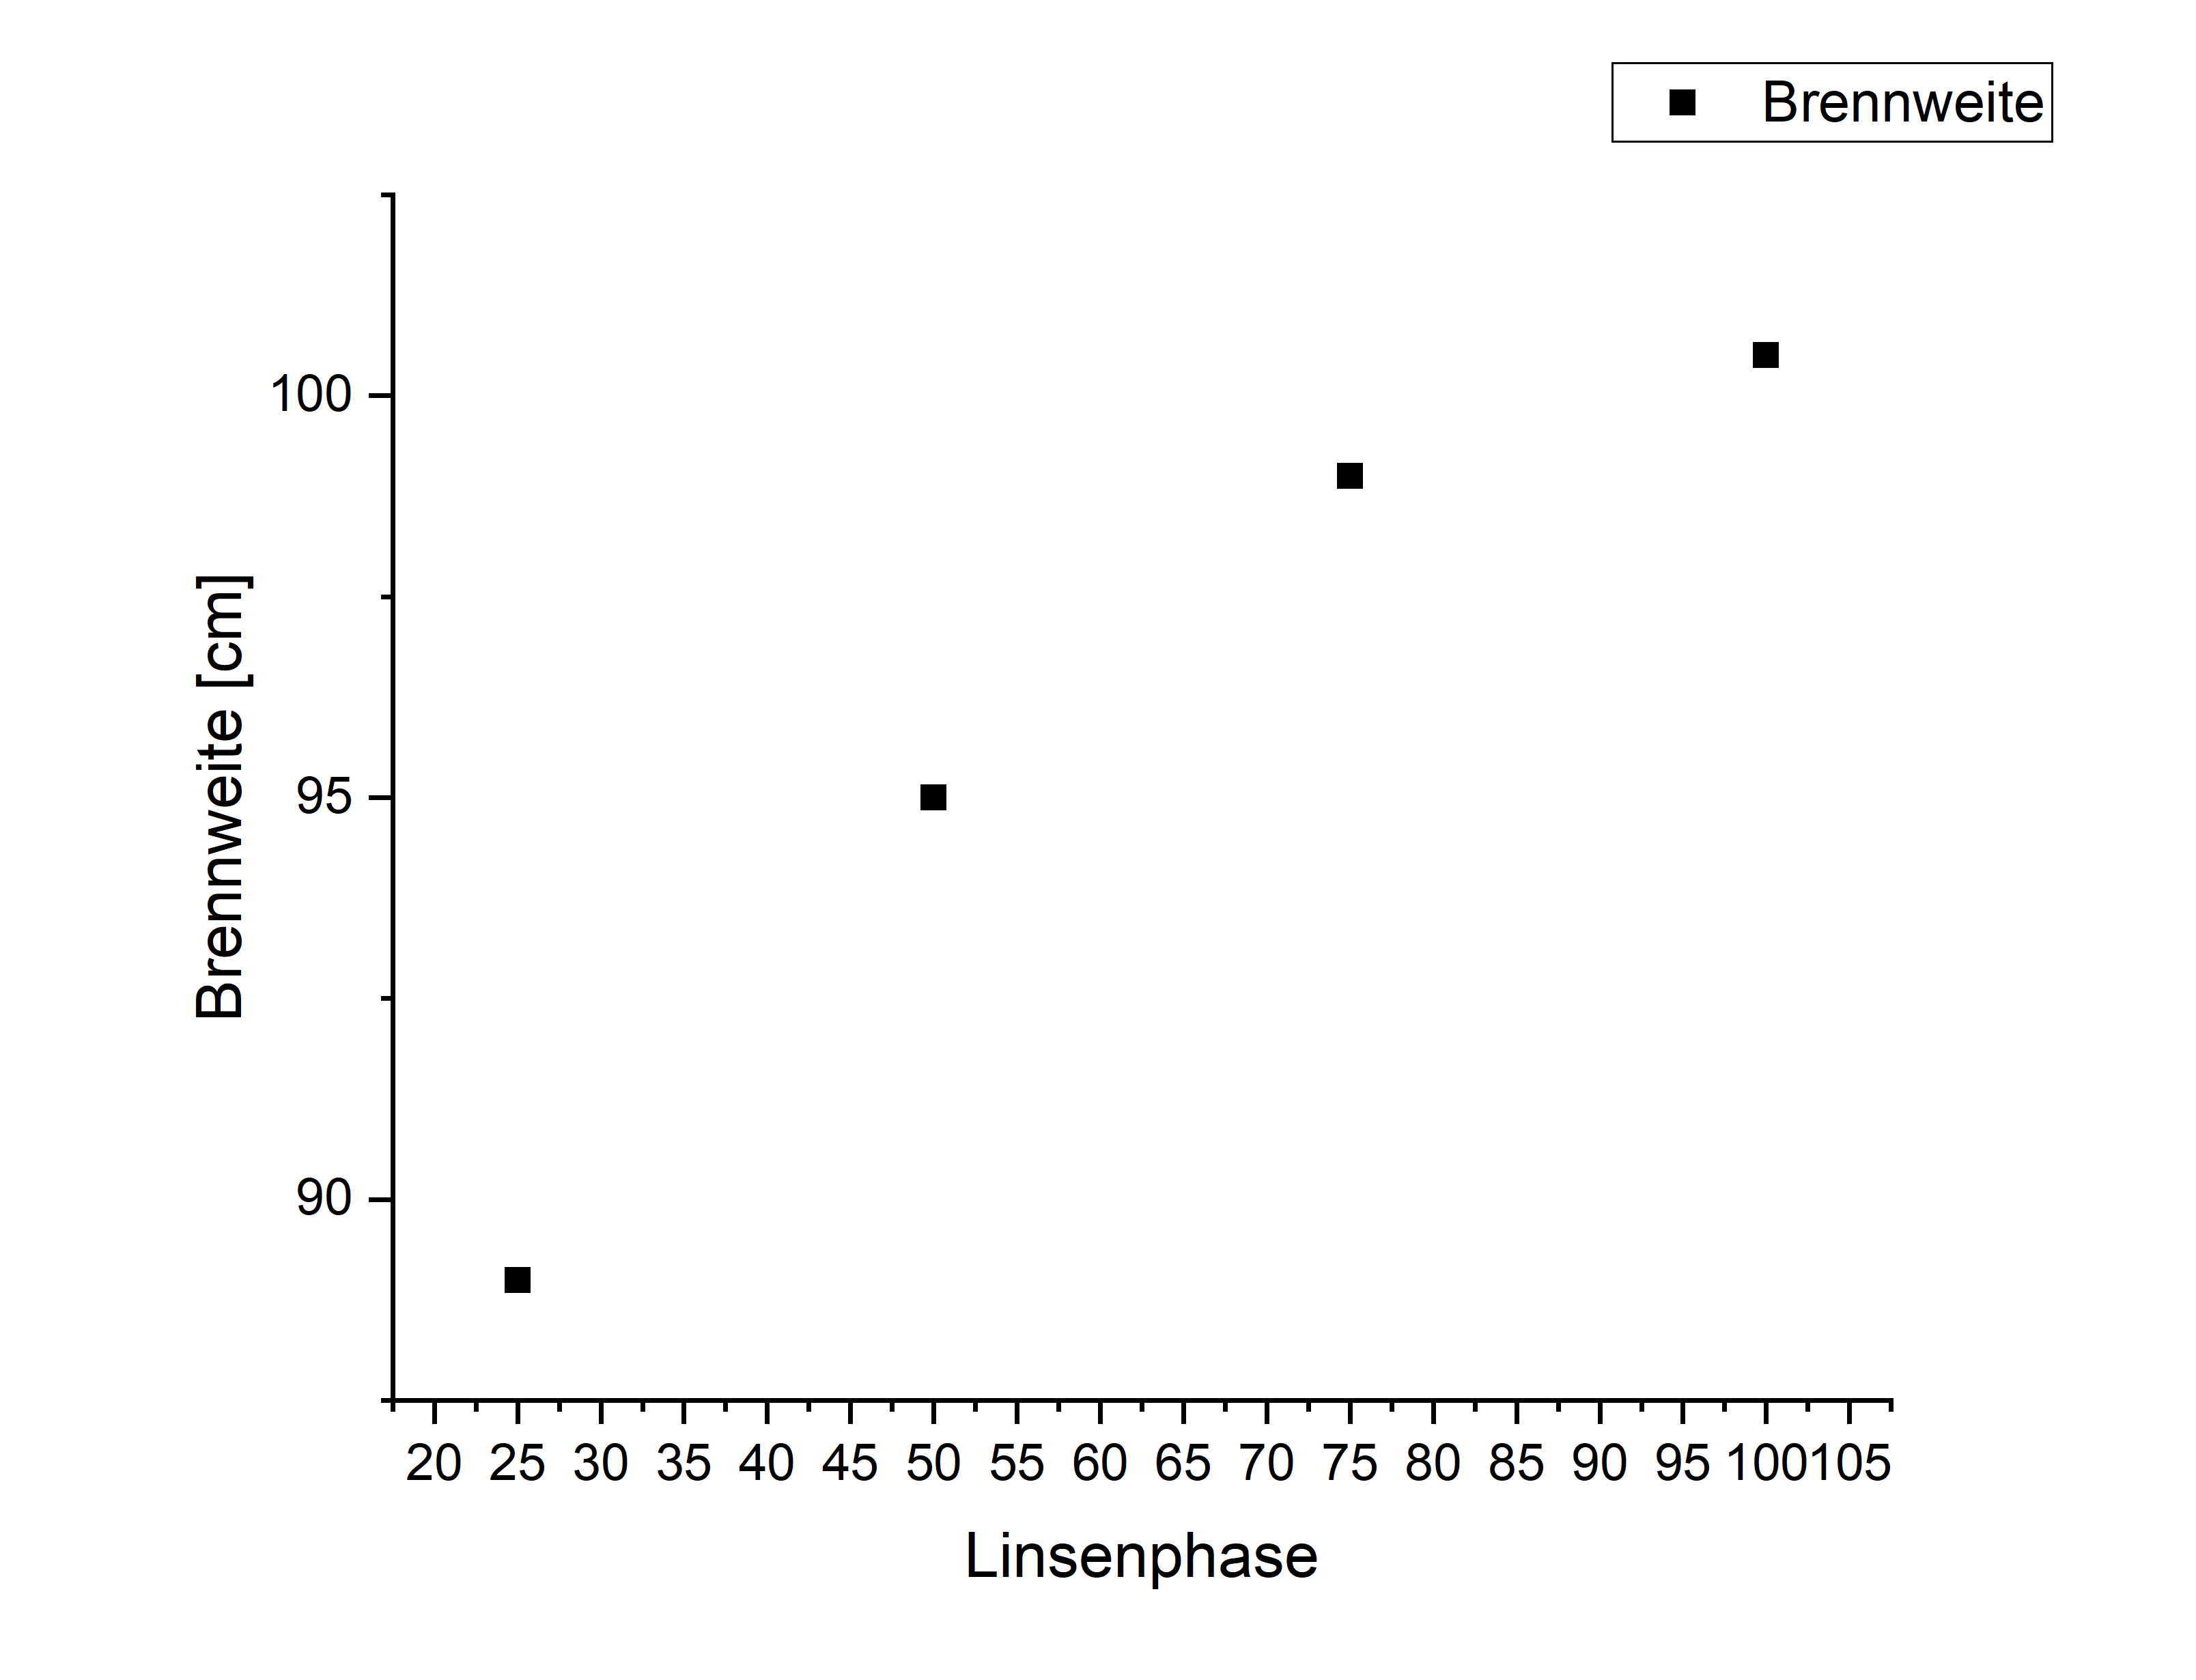
\includegraphics[width=0.9\textwidth]{linsenphase.png}
	\caption{Die Brennweite in cm aufgetragen gegen die eingestellte Linsenphase. Die wurzelförmige Abhängigkeit ist deutlich erkennbar.}
	\label{linsenphase}
\end{figure}

\subsection{Berechnung beliebiger diffraktiver optischer Elemente als CGH}
Mit Hilfe der OptiXplorer Sofware können ebenfalls Hologramme erzeugt werden. Dazu wird zunächst ein Bild aus den vorgegebenen Beispielbildern ausgesucht. Durch die gegebene Funktion "generate CGH" kann der sogenannte Iterative Fourier-Transformations-Algorithmus ausgeführt werden. Das Bild wird an den LC-Modulator übergeben, mit dem Laser durchleuchtet und anschließend mit einer Kamera aufgenommen und gespeichert. Danach wird der selbe Vorgang mit einem weiteren Beispielbild wiederholt. In  \cref{hologram} sind die beiden mit Hilfe der Kamera aufgenommenen Bilder zu sehen. Man erkennt, dass die Beispielbilder, die auf den LC-Modulator geschickt wurden, mit hoher Genauigkeit wiedergegeben wurden. Die Holografie funktioniert aufgrund der zugrundeliegenden Beugungstheorie, welche besagt, dass durch eine Fouriertransformation das Bild rekonstruiert werden kann.

\begin{figure}[h]
	\begin{subfigure}[c]{0.5\textwidth}
		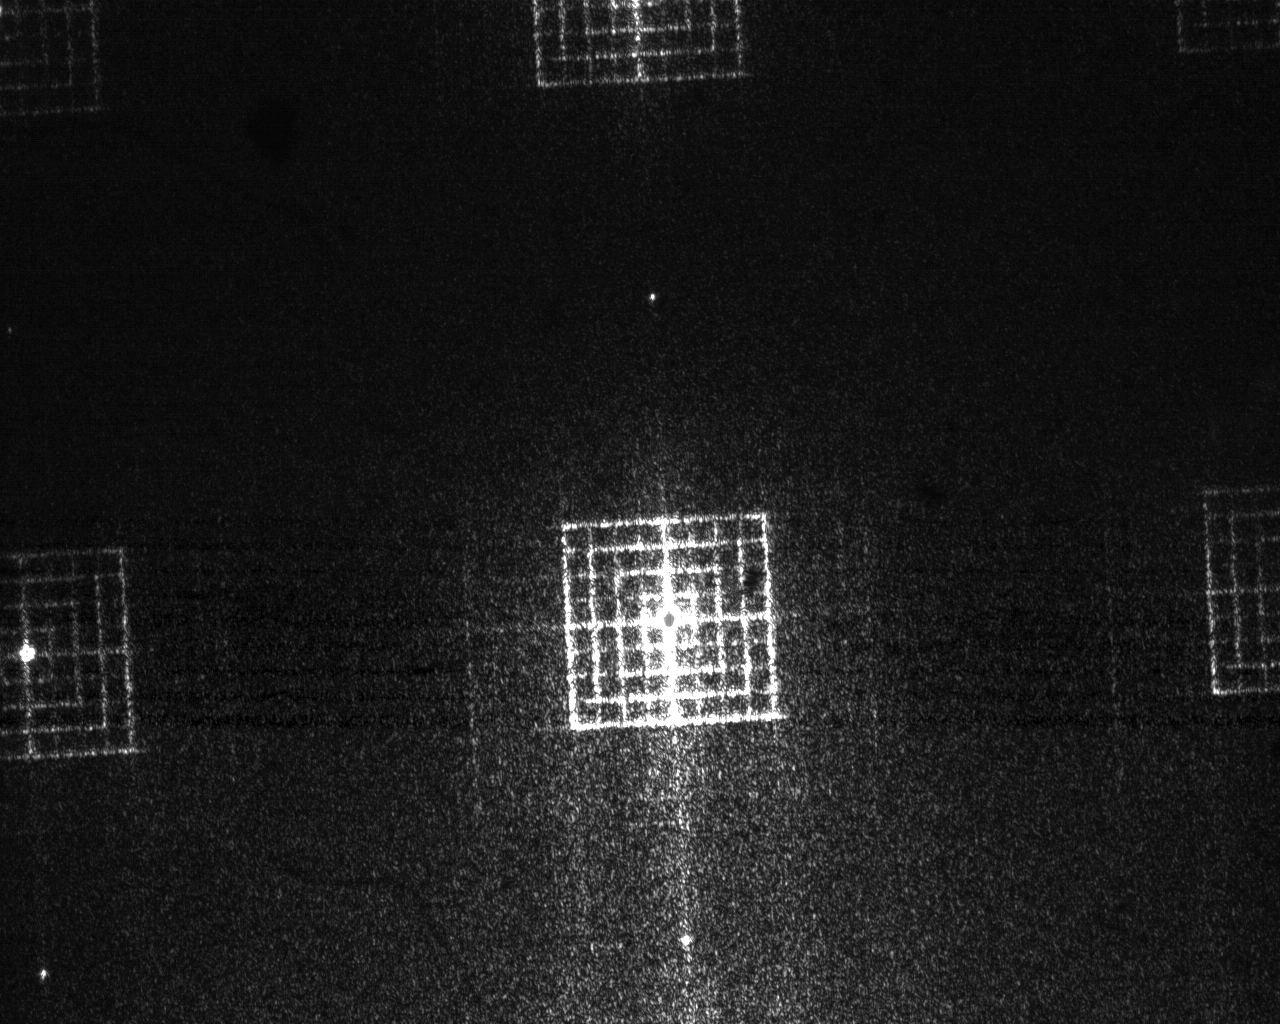
\includegraphics[width=0.9\textwidth]{Holo1.png}
		
	\end{subfigure}
	\begin{subfigure}[c]{0.5\textwidth}
		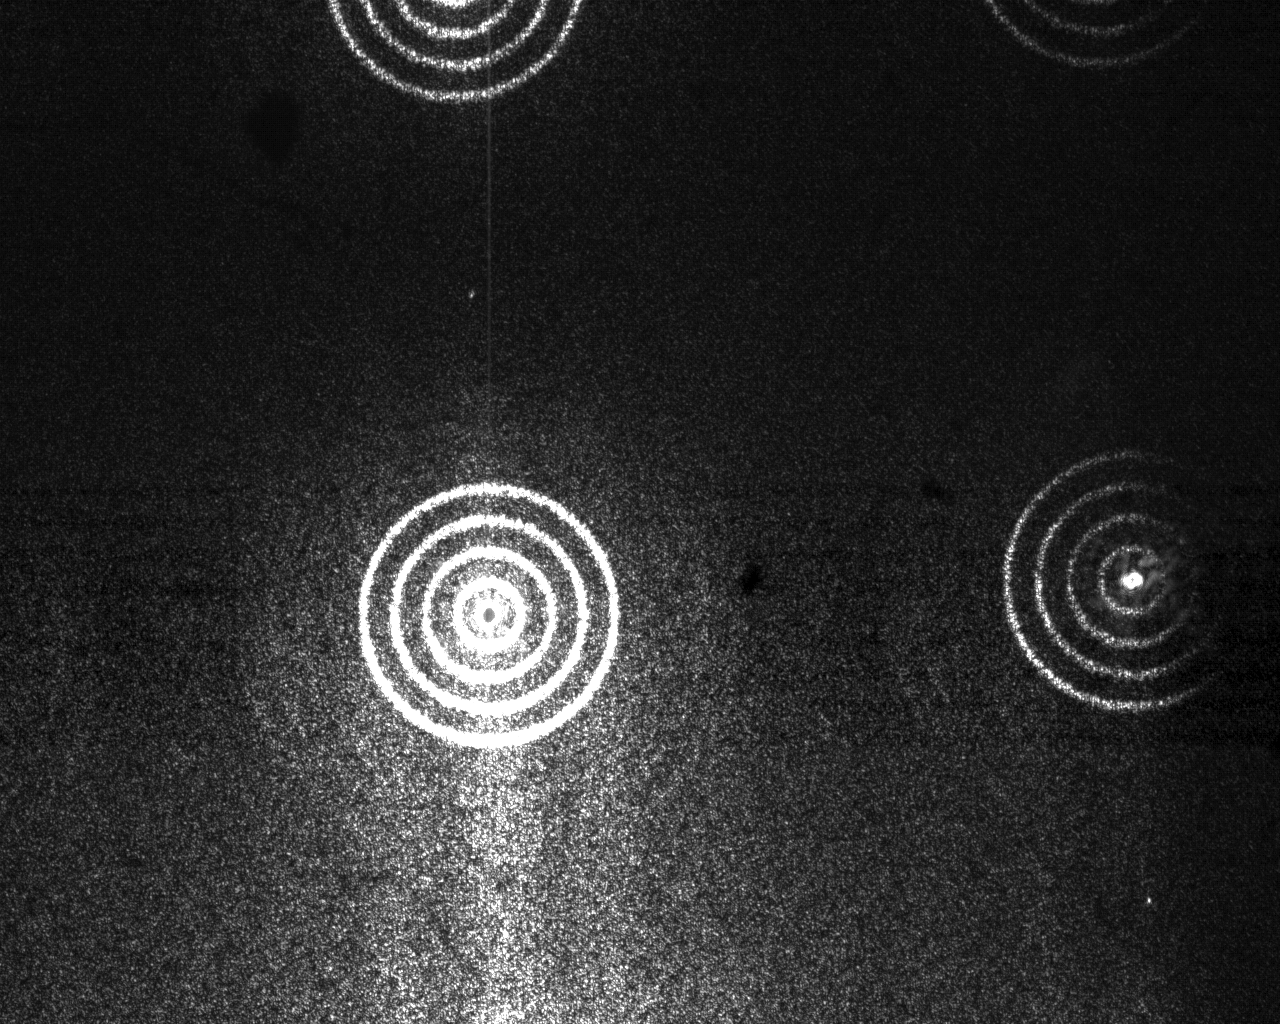
\includegraphics[width=0.9\textwidth]{Holo2.png}
	\end{subfigure}
	\caption{Zwei computergenerierte Hologramme, die mit "generate CHG" der OptiXplorer Software erstellt wurden.}
	\label{hologram}
\end{figure}

\subsection{Darstellung zweier DOEs auf einem Bildschirm}
Im letzten Versuchsteil wird untersucht, was passiert, wenn beide vorher erstellten Hologramme gleichzeitig erzeugt werden. Hierfür werden beide jeweils auf die Hälfte des Bildschirms projeziert. In \cref{holo2} ist das mit Hilfe der Kamera aufgenommene Bild der Überlagerung zweier DOE’s zu sehen. Es sind beide Muster klar erkennbar, jedoch liegen die Bilder nicht nebeneinander, wie man zunächst vermuten könnte, sondern übereinander. Dies folgt aus der doppelten Fouriertransformation. Da diese das im Ortsraum befindliche Bild in den Frequenzraum transformiert und andersherum, werden dabei die Frequenzen überlagert und nicht wie im Ortsraum ursprünglich räumlich getrennt gesehen. Werden dann die überlagerten Frequenzen zurück in den Ortsraum transformiert, erhält man nicht mehr das räumlich getrennte Bild von Ringen und Quadraten, sondern eine Überlagerung der beiden Bilder.

\begin{figure}
	\centering
	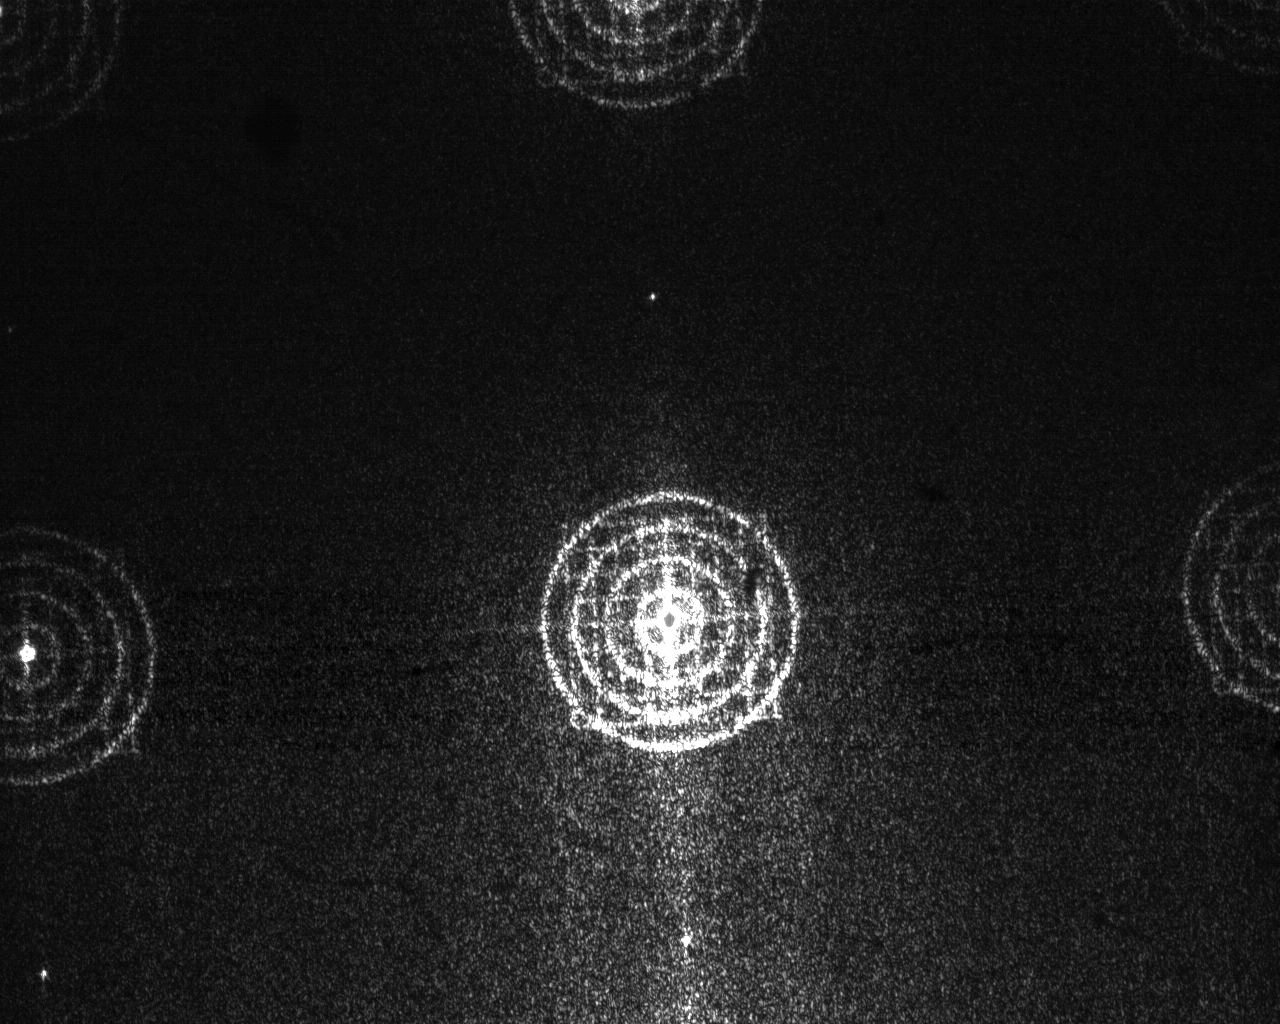
\includegraphics[width=0.9\textwidth]{holobeide.png}
	\caption{Das mit der Kamera aufgezeichnete Bild, wenn beide Hologramme gleichzeitig nebeneinander erzeugt werden.}
	\label{holo2}
\end{figure}


